\documentclass[12pt,a4]{article}










\usepackage{graphicx,amsmath,amssymb,amsthm, boxedminipage,xcolor,amscd,amsbsy,latexsym,url,bm}

%\usepackage[lined,boxed]{algorithm2e}

\usepackage{algorithm}
\usepackage{algpseudocode}


\newtheorem{theorem}{Theorem}[section]
\newtheorem{proposition}[theorem]{Proposition}
\newtheorem{lemma}[theorem]{Lemma}
\newtheorem{corollary}[theorem]{Corollary}
\newtheorem{definition}[theorem]{Definition}

\newtheorem*{theorem*}{Theorem}
\newtheorem*{lemma*}{Lemma}
\newtheorem*{solution}{Solution}
\newtheorem*{proposition*}{Proposition}


\newtheorem{exercise}[theorem]{Exercise}
\newtheorem{exerciseD}[theorem]{*Exercise}
\newtheorem{exerciseDD}[theorem]{**Exercise}

\let\oldexercise\exercise
\renewcommand{\exercise}{\oldexercise\normalfont}

\let\oldexerciseD\exerciseD
\renewcommand{\exerciseD}{\oldexerciseD\normalfont}

%\let\oldexerciseD\exerciseD
%\renewcommand{\exerciseD}{\oldexerciseD\normalfont}

%\let\oldexerciseDD\exerciseDD
%\renewcommand{\exerciseDD}{\oldexerciseDD\normalfont}

\newcommand{\E}{\mathbb{E}}
%\newcommand{\nth}[1]{#1^{\textsuperscript{th}}}
\newcommand{\scalar}[2]{\ensuremath{\langle #1, #2\rangle}}
\newcommand{\floor}[1]{\left\lfloor #1 \right\rfloor}
\newcommand{\ceil}[1]{\left\lceil #1 \right\rceil}
\newcommand{\norm}[1]{\|#1\|}
\newcommand{\pfrac}[2]{\left(\frac{#1}{#2}\right)}
\newcommand{\nth}[1]{#1^{\textsuperscript{th}}}
\newcommand{\core}{\textnormal{core}}



\newif\ifsolution

\solutionfalse

\newcommand{\answer}[1]{
\ifsolution
{\color{blue} #1}
\else
\fi
}



\newcommand{\poly}{\textnormal{poly}}
\newcommand{\quasipol}{\textnormal{quasipol}}
\newcommand{\ssubexp}{\textnormal{stronglySubExp}}
\newcommand{\wsubexp}{\textnormal{weaklySubExp}}
\newcommand{\simplyexp}{\textnormal{E}}
\newcommand{\expo}{\textnormal{Exp}}



\newcommand{\N}{\mathbb{N}}
\newcommand{\nn}{\mathbb{N}_0^n}
\newcommand{\R}{\mathbb{R}}
\newcommand{\Z}{\mathbb{Z}}


\definecolor{darkgreen}{rgb}{0,0.6,0}

\date{}

\title{
\hbox{  Mathematical Foundations of Computer Science}
  \vspace{3mm}
{\normalsize CS 499,	Shanghai Jiaotong University,  Dominik Scheder\\
%\vspace{3mm}
Spring 2019}
}


\begin{document}

\maketitle

%\begin{quotation}
%  You are welcome to discuss the exercises in the discussion
%  forum. Please take them serious. Doing the exercises is as important
%  than watching the videos.
%
%  I intentionally included very challenging exercises and marked them
%  with one or two ``$*$''. No star means you should be able to solve
%  the exercises without big problems once you have understood
%  the material from the video lecture. One star means it requires 
%  significant additional thinking. Two stars means it is not 
%  unlikely that you will fail to solve them, even once you have understood
%  the material and thought a lot about the exercise. Don't feel bad
%  if you fail. Failure is part of learning.
%
%  This is the first time this course is online. Thus there might be mistakes
%  (typos or more serious conceptual mistakes) in the exercises. I will be 
%  grateful if you point them out to me!
%\end{quotation}


\begin{document}

\maketitle

%\begin{quotation}
%  You are welcome to discuss the exercises in the discussion
%  forum. Please take them serious. Doing the exercises is as important
%  than watching the videos.
%
%  I intentionally included very challenging exercises and marked them
%  with one or two ``$*$''. No star means you should be able to solve
%  the exercises without big problems once you have understood
%  the material from the video lecture. One star means it requires 
%  significant additional thinking. Two stars means it is not 
%  unlikely that you will fail to solve them, even once you have understood
%  the material and thought a lot about the exercise. Don't feel bad
%  if you fail. Failure is part of learning.
%
%  This is the first time this course is online. Thus there might be mistakes
%  (typos or more serious conceptual mistakes) in the exercises. I will be 
%  grateful if you point them out to me!
%\end{quotation}




\setcounter{section}{2}

\begin{center}
  \large\textbf{Group: navigator} 
\end{center}
\begin{center}
  \begin{tabular}{rl}
 Xu Huan  & 517021910724 \\
 Tianyao Shi     &     517021910623 \\
Chenxiao Yang    &    517021910540  \\
Jiaqi  Zng      &     517021910882  \\
  \end{tabular}
\end{center}

\newpage


\section{Tossing Coins}

Let us toss a coin infinitely often, producing a bit string $x = x_1 x_2 x_3 \dots$. For a finite bit string $z \in \{0,1\}^*$, let $T_z$ denote the number of tosses
until $z$ appears the first time. For example, if we toss $0010110$, then $T_{10} = 4$ and
$T_{110} = 7$.

\begin{exercise}
   Consider an unbiased coin, i.e., $0$ and $1$ come up with probability $p=1/2$ each.
   \begin{enumerate}
        \item Give an explicit\footnote{By {\em explicit} in this context I mean something
        not containing a recurrence; not containing $\sum$ or $\prod$. You may, however,
        use stuff we have used before, like ${n \choose k}$, Fibonacci numbers $F_n$,
        Catalan numbers $C_n$.}
         formula for $\Pr[T_{10} = n]$.
        \item Give an explicit formula for $\Pr[T_{11} = n]$. 
       \item  Compute $\E[T_{11}]$ and $\E[T_{10}]$. You can choose any of the three proof methods above (but 
   two of them won't be fun; in particular, using Point 1 and Point 2 of this exercise will not help you so much).
   \end{enumerate} 
\end{exercise}

%----------------------------3.1.1----------------------------
\begin{solution} \quad
      \begin{enumerate}
         \item Consider a string that does not contain any ``$10$'' in first $n$ tosses. Let us denote the string as $B_n$, and analyse the form it should take.
         \begin{itemize}
            \item If $B_n$ starts with a `$0$', then the next bit of the string can be either a `$0$' or `$1$'. In other words, the following $n-1$ bits can be any specific element in $B_{n-1}$.
            \item If $B_n$ starts with a `$1$', then the next bit can only be `$1$' as $B_n$ does not contain ``$10$''. Like wise, the second, third, \dots bit can only be `$1$' as well. The only possible form for $B_n$ starting with `$1$' is a string that only contains `$1$'.
         \end{itemize}
         From the two cases we can conclude that $$B_n=\{\{0,1\}^n|0x,x\in B_{n-1}\;\text{or}\;111\cdots1\},$$ and derive that 
         $$
         |B_n|=|B_{n-1}|+1.
         $$
         We have $|B_1|=2$ and $|B_2|=3$, from which we can easily get that $|B_n|=n+1$.

         Back to our problem, the event $T_{10}=n$ refers to such string $S_n$ that $$S_n=\{\{0,1\}^n|y10,y\in B_{n-2}\},$$ for which we have $$|S_n|=|B_{n-2}|=n-1.$$
        Therefore we have $$\Pr[T_{10} = n]=\frac{n-1}{2^n}.$$

%----------------------------3.1.2----------------------------
        \item The event $T_{11}=n$ refers to such string $S_n$ that $$S_n=\{\{0,1\}^n|z011,z\in A_{n-3}\},$$ for which we have $$|S_n|=|A_{n-3}|=F_{n-1}.$$
        Therefore we have $$Pr[T_{11}=n]=\frac{F_{n-1}}{2^n}.$$

%----------------------------3.1.3----------------------------      
        \item Since you have just implied the first two points won't be fun, let us just try with the automaton, which is shown in Figure~\ref{Fig-3.1}. For every transmitting line, the corresponding probability is $p=1/2$ as this is an unbiased coin.
        
         For solving $\E[T_{10}]$, see Figure~\ref{Fig-3.1}(a), from which we can derive
         \begin{align*}
            \E[T_{10}]=\E[a]&=1+\frac{1}{2}\E[a]+\frac{1}{2}\E[b],\\
            \E[b]&=1+\frac{1}{2}\cdot0+\frac{1}{2}\E[c],\\
            \E[c]&=1+\frac{1}{2}\cdot0+\frac{1}{2}\E[c],
         \end{align*}
         where state $a$ can been seen as the initial state, and $\E[a]$ means the expectation of number of tosses from state $a$ till the pattern ``$10$'' appears. State $d$ is the final state, therefore having $\E[d]=0$. By solving these equations, we get $\E[T_{10}]=4$.
        \begin{figure}[htbp]
         \captionsetup{skip=2pt}
         \vspace{0pt}
         \begin{subfigure}{.5\textwidth}
             \centering
             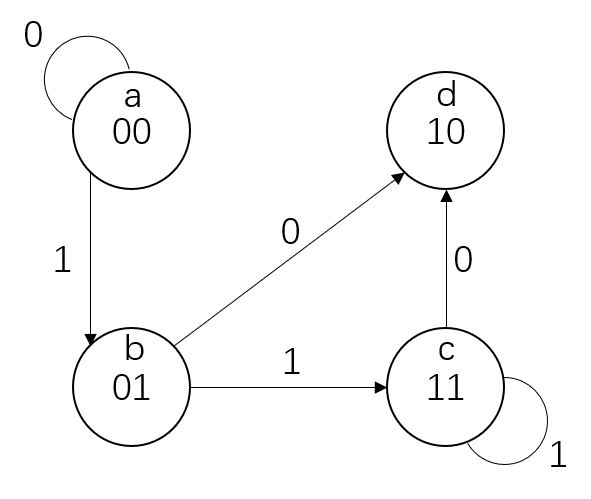
\includegraphics[width=\textwidth]{figures/Fig-3-1a.PNG}
             \caption{}
         \end{subfigure}
         \begin{subfigure}{.5\textwidth}
             \centering
             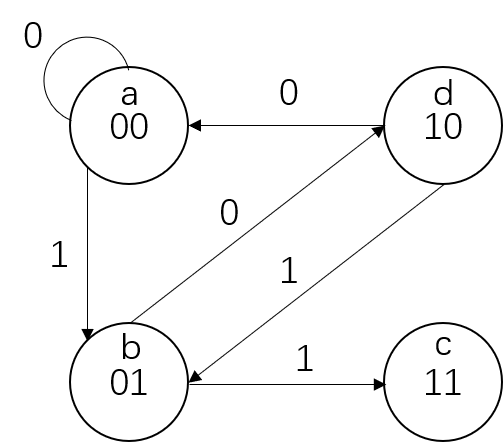
\includegraphics[width=0.85\textwidth]{figures/Fig-3-1b.PNG}
             \caption{}
         \end{subfigure}
         \caption{Automatons for two different finishing states}\label{Fig-3.1}
     \end{figure}
     
     For solving $\E[T_{11}]$, see Figure~\ref{Fig-3.1}(b), from which we can derive
         \begin{align*}
            \E[T_{11}]=\E[a]&=1+\frac{1}{2}\E[a]+\frac{1}{2}\E[b],\\
            \E[b]&=1+\frac{1}{2}\cdot0+\frac{1}{2}\E[d],\\
            \E[d]&=1+\frac{1}{2}\E[a]+\frac{1}{2}\E[b],
         \end{align*}
         where state $a$ can been seen as the initial state, and $\E[a]$ means the expectation of number of tosses from state $a$ till the pattern ``$11$'' appears. State $c$ is the final state, therefore having $\E[c]=0$. By solving these equations, we get $\E[T_{11}]=6$.
      \end{enumerate}
   \end{solution}

You might have noticed that $\E[T_{10}] < \E[T_{11}]$, i.e., $10$ appears earlier than $11$, on average.
\begin{exercise}
   Let $\mathcal{E}$ be the event that $10$ appears earlier than $11$. What is $\Pr[\mathcal{E}]$?
\end{exercise}

%----------------------------3.2----------------------------
\begin{solution}
The 4 possible status and there conversion relationship are shown as the following picture.
\begin{figure}[htbp]
    \centering
    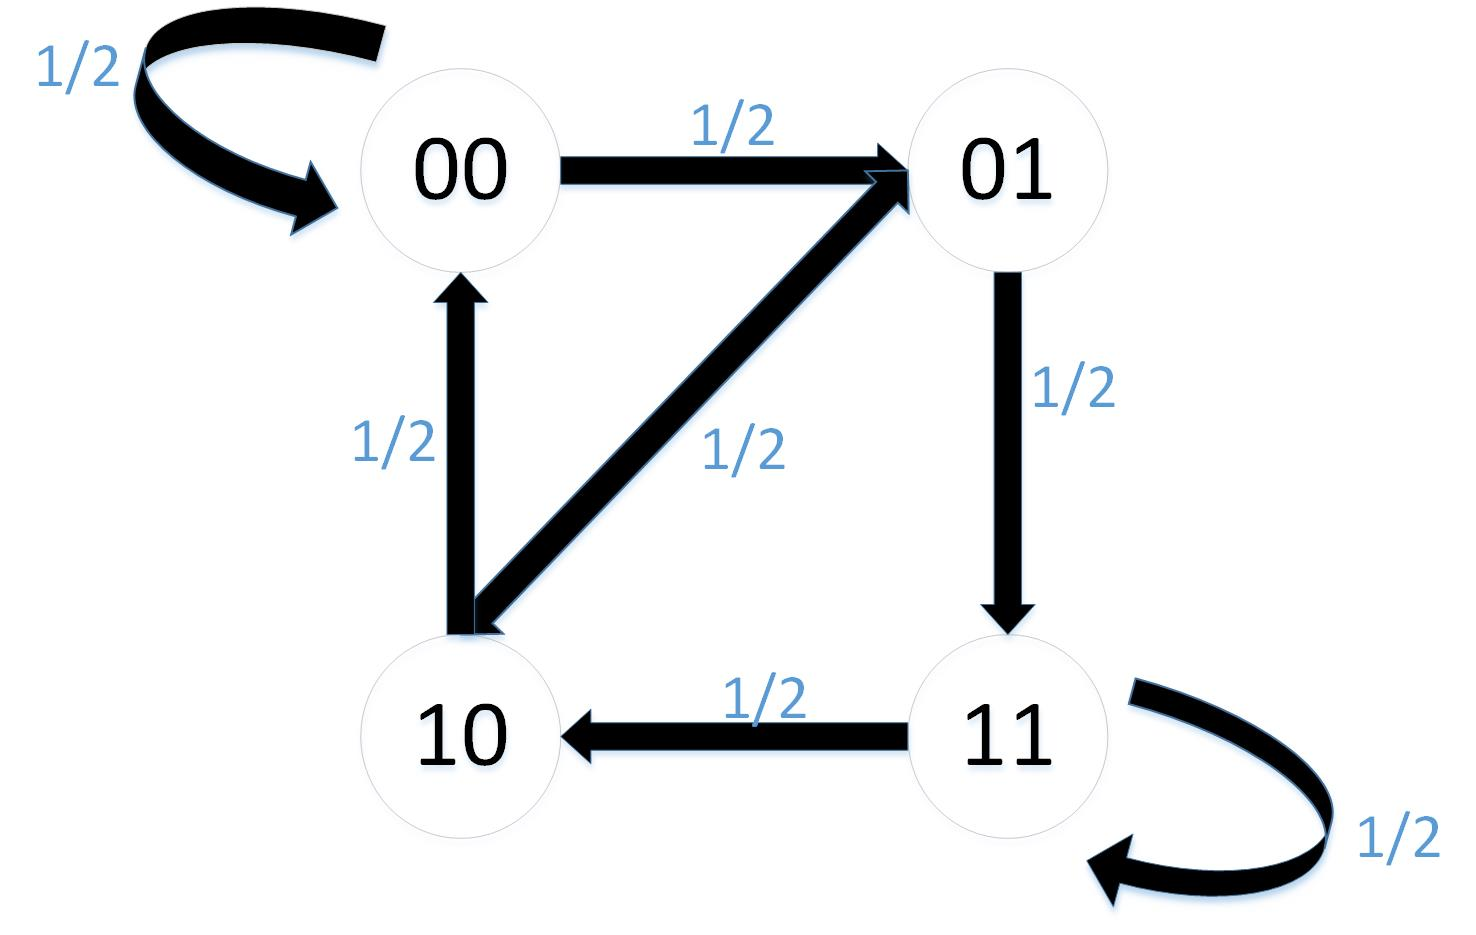
\includegraphics[width=0.5\textwidth]{figures/1.jpg}
    \caption{Recurrence Tree}\label{tree}
\end{figure}
To reach the status \textit{11} or \textit{10}, we should first reach status \textit{01}. From the picture we can know that the possibility from status \textit{01} to status \textit{11} and \textit{10} are equal, which means that the $Pr[10 \, appears \, earlier]=Pr[11 \, appears \,  earlier]=\frac{1}{2}$.
\end{solution}

\begin{exercise}
   Toss two coins repeatedly, producing two sequences $x_1 x_2 \dots$ and $y_1 y_2 \dots$.
   We stop once we see $10$ in the first sequence or $11$ in the second sequence. Formally,
   we toss the two coins
   \begin{align*}
      T:=  \min (T_{10}(x), T_{11}(y)) 
   \end{align*}   
   times.
   \begin{enumerate}
     \item What is $\E[T]$?
     \item What are the probabilities that $10$ appears in $x$ (a) before $11$ appears in $y$, (b) at the same time as $11$,
     (c) later than $11$?
     \end{enumerate}
     \textbf{Hint.} I think the only way to solve this exercise without going crazy is by applying proof method 3 
     from above, drawing a small automaton; or in this case, not so extremely small anymore.
\end{exercise}

%----------------------------3.3.1----------------------------
\begin{solution} \quad
  \begin{enumerate}
    \item
  Draw an automaton as shown. Every state is $2 \times 2$, of which the two rows respectively denote the last two bits of the sequences $x_1 x_2 \dots$ and $y_1 y_2 \dots$. The state {\color{red}{T}} denotes either of the two sequences reaches termination condition, i.e. 10 appears in $x$ sequence or 11 appears in $y$ sequence. Name these states from $s_1, s_2, \cdots, s_9$.\par
  \begin{center}
    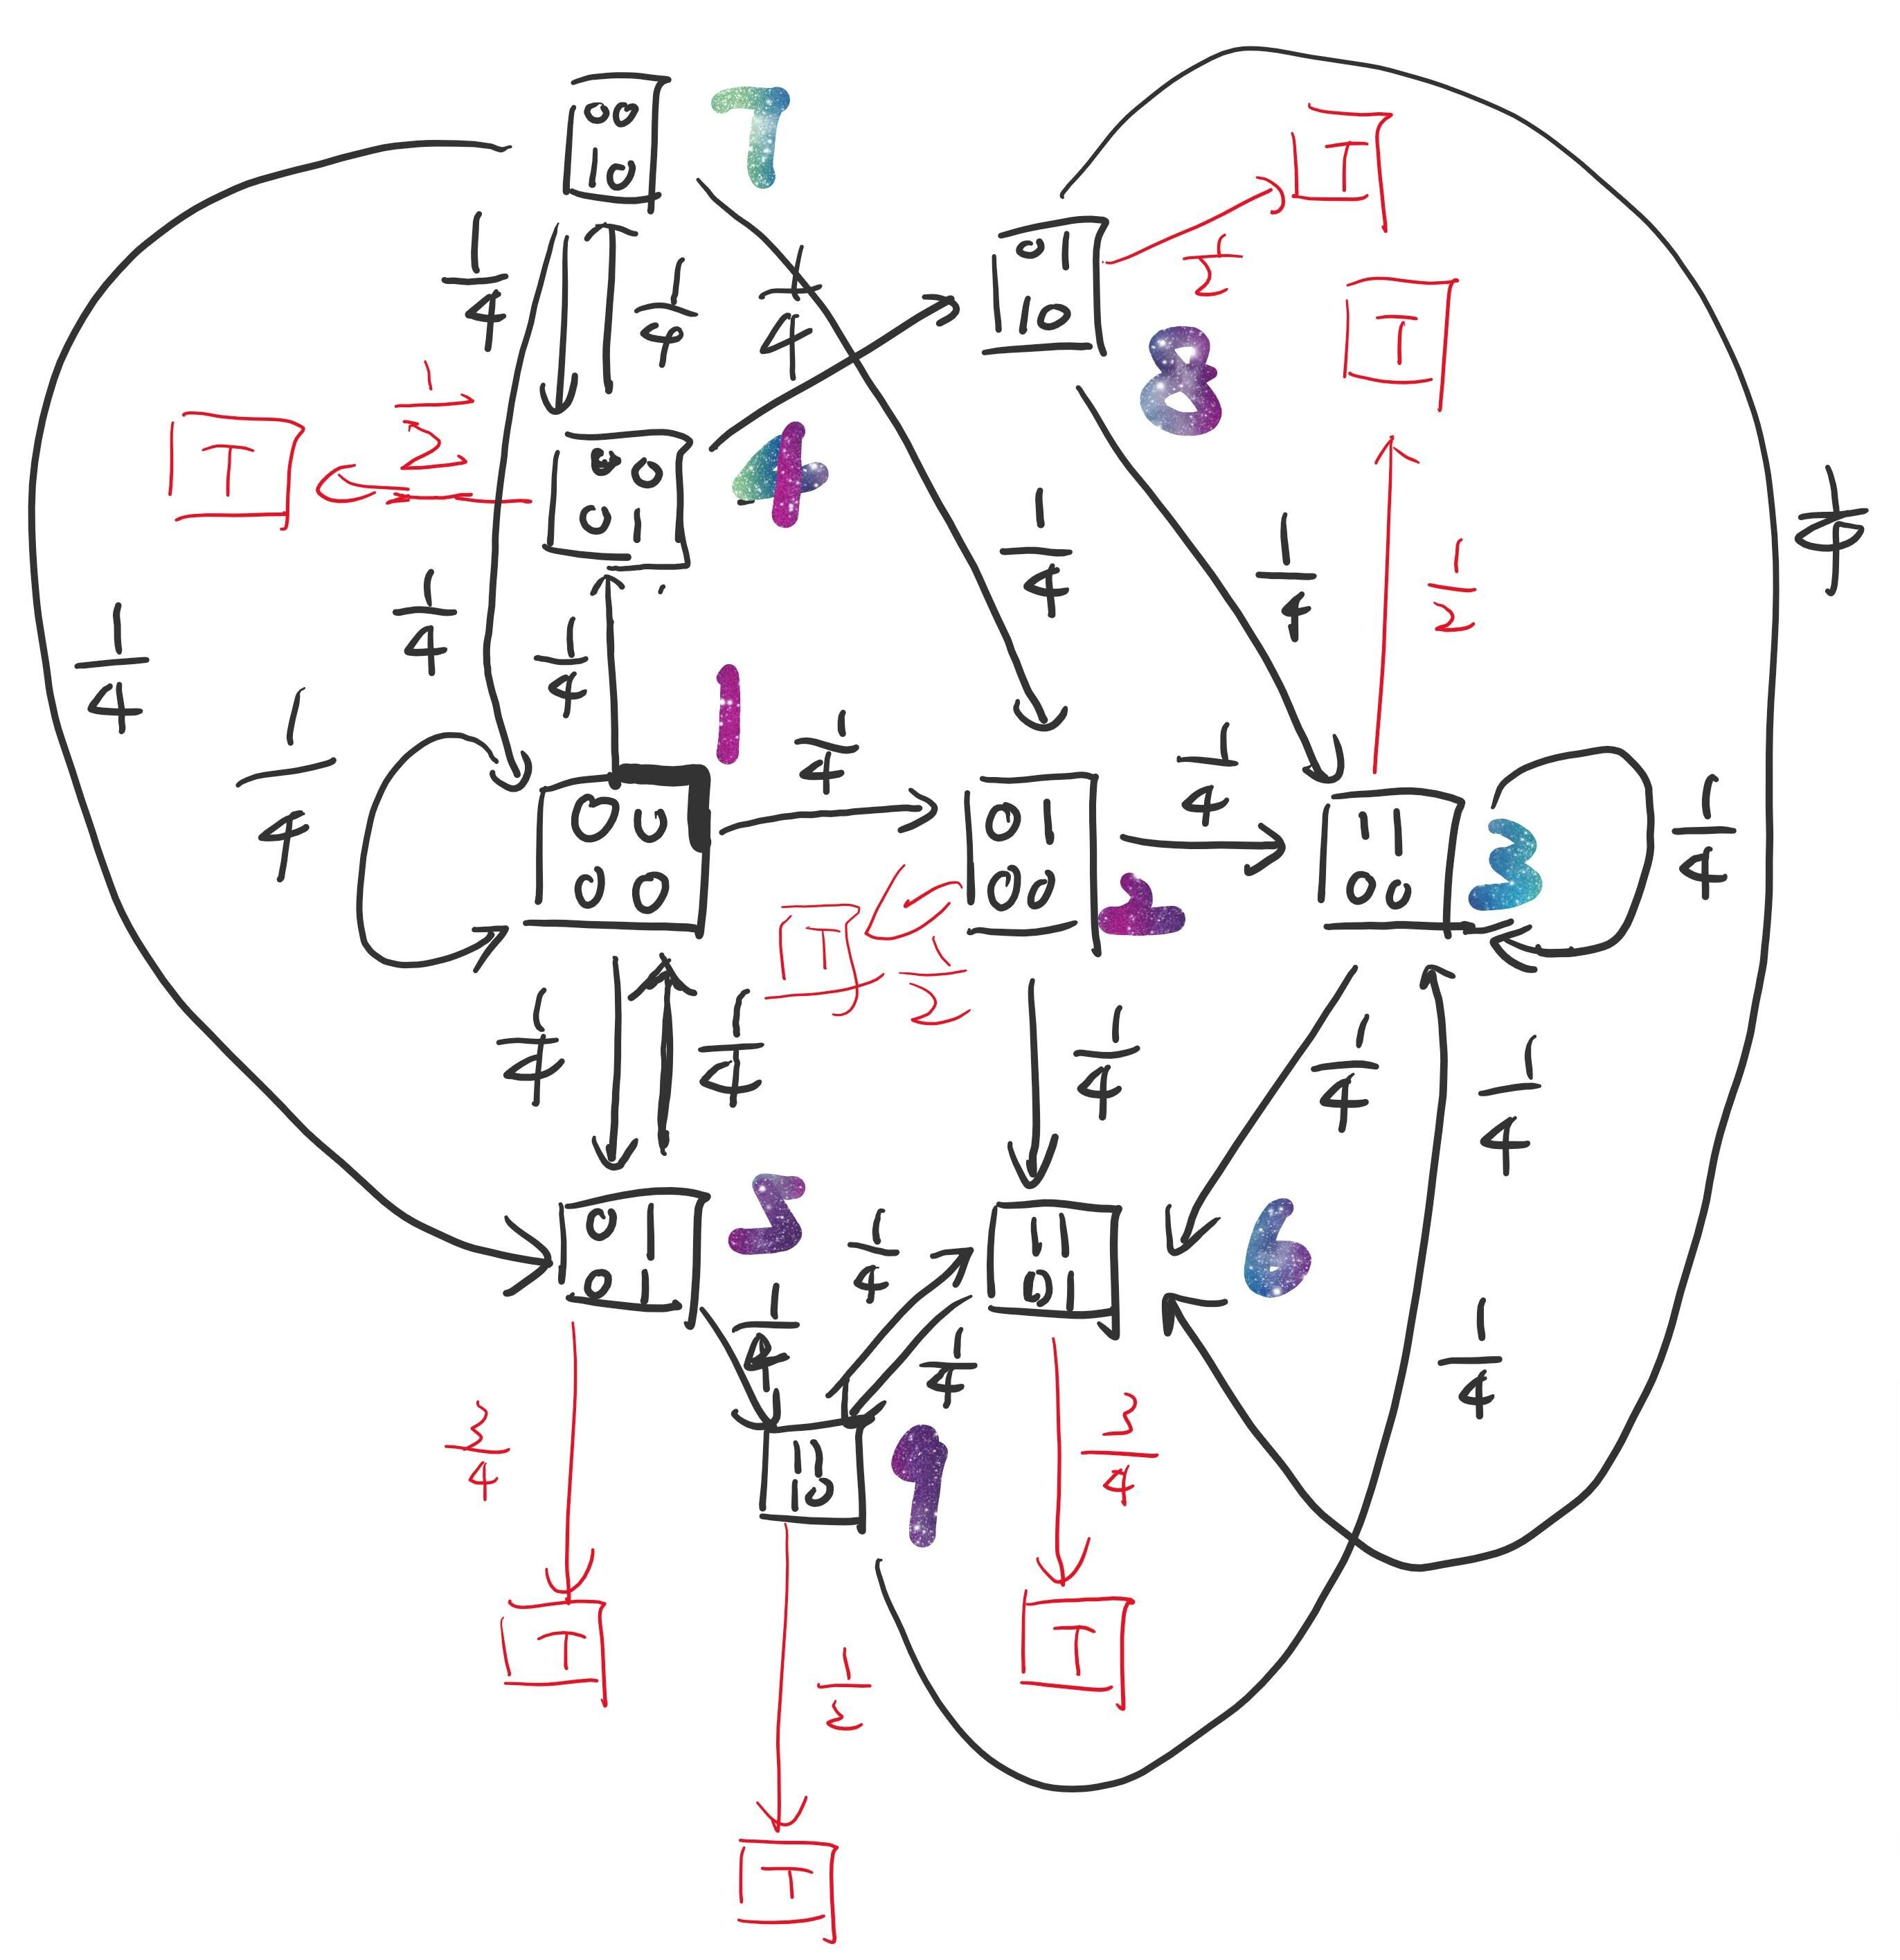
\includegraphics[width=0.6\textwidth]{figures/e33_p1.jpg}
  \end{center}
  Then we can create a $9 \times 9$ Markov matrix $A^{(9)}$ to denote this automaton.
  $$
  A^{(9)} = \frac{1}{4} \times 
  \bordermatrix{&1 &2 &3 &4 &5 &6 &7 &8 &9 \cr
              1 &1 &1 &  &1 &1 &  &  &  &  \cr
              2 &  &  &1 &  &  &1 &  &  &  \cr
              3 &  &  &1 &  &  &1 &  &  &  \cr
              4 &  &  &  &  &  &  &1 &1 &  \cr
              5 &  &  &  &  &  &  &  &  &1 \cr
              6 &  &  &  &  &  &  &  &  &1 \cr
              7 &1 &1 &  &1 &1 &  &  &  &  \cr
              8 &  &  &1 &  &  &1 &  &  &  \cr
              9 &  &  &1 &  &  &1 &  &  &  \cr
  }
  $$
  $$a_{ij} = 
  \begin{cases}
  0 & P_r(s_i \rightarrow s_j) = 0 \\
  1 & P_r(s_i \rightarrow s_j) = \frac{1}{4}
  \end{cases}$$
  Observation: some of the rows are just the same e.g. $r_1 \& r_7$, thus they can be merged. Then we have a merged matrix $B^{(4)}$.
  $$
  B = \frac{1}{4} \times 
  \bordermatrix{&1 &2 &4 &5 \cr
              1 &1 &1 &1 &1 \cr
              2 &  &1 &  &1 \cr
              4 &1 &1 &  &  \cr
              5 &  &1 &  &  \cr
  }
  $$
  According to matrix $B$, we can create a simplified automaton as shown.
  \begin{center}
   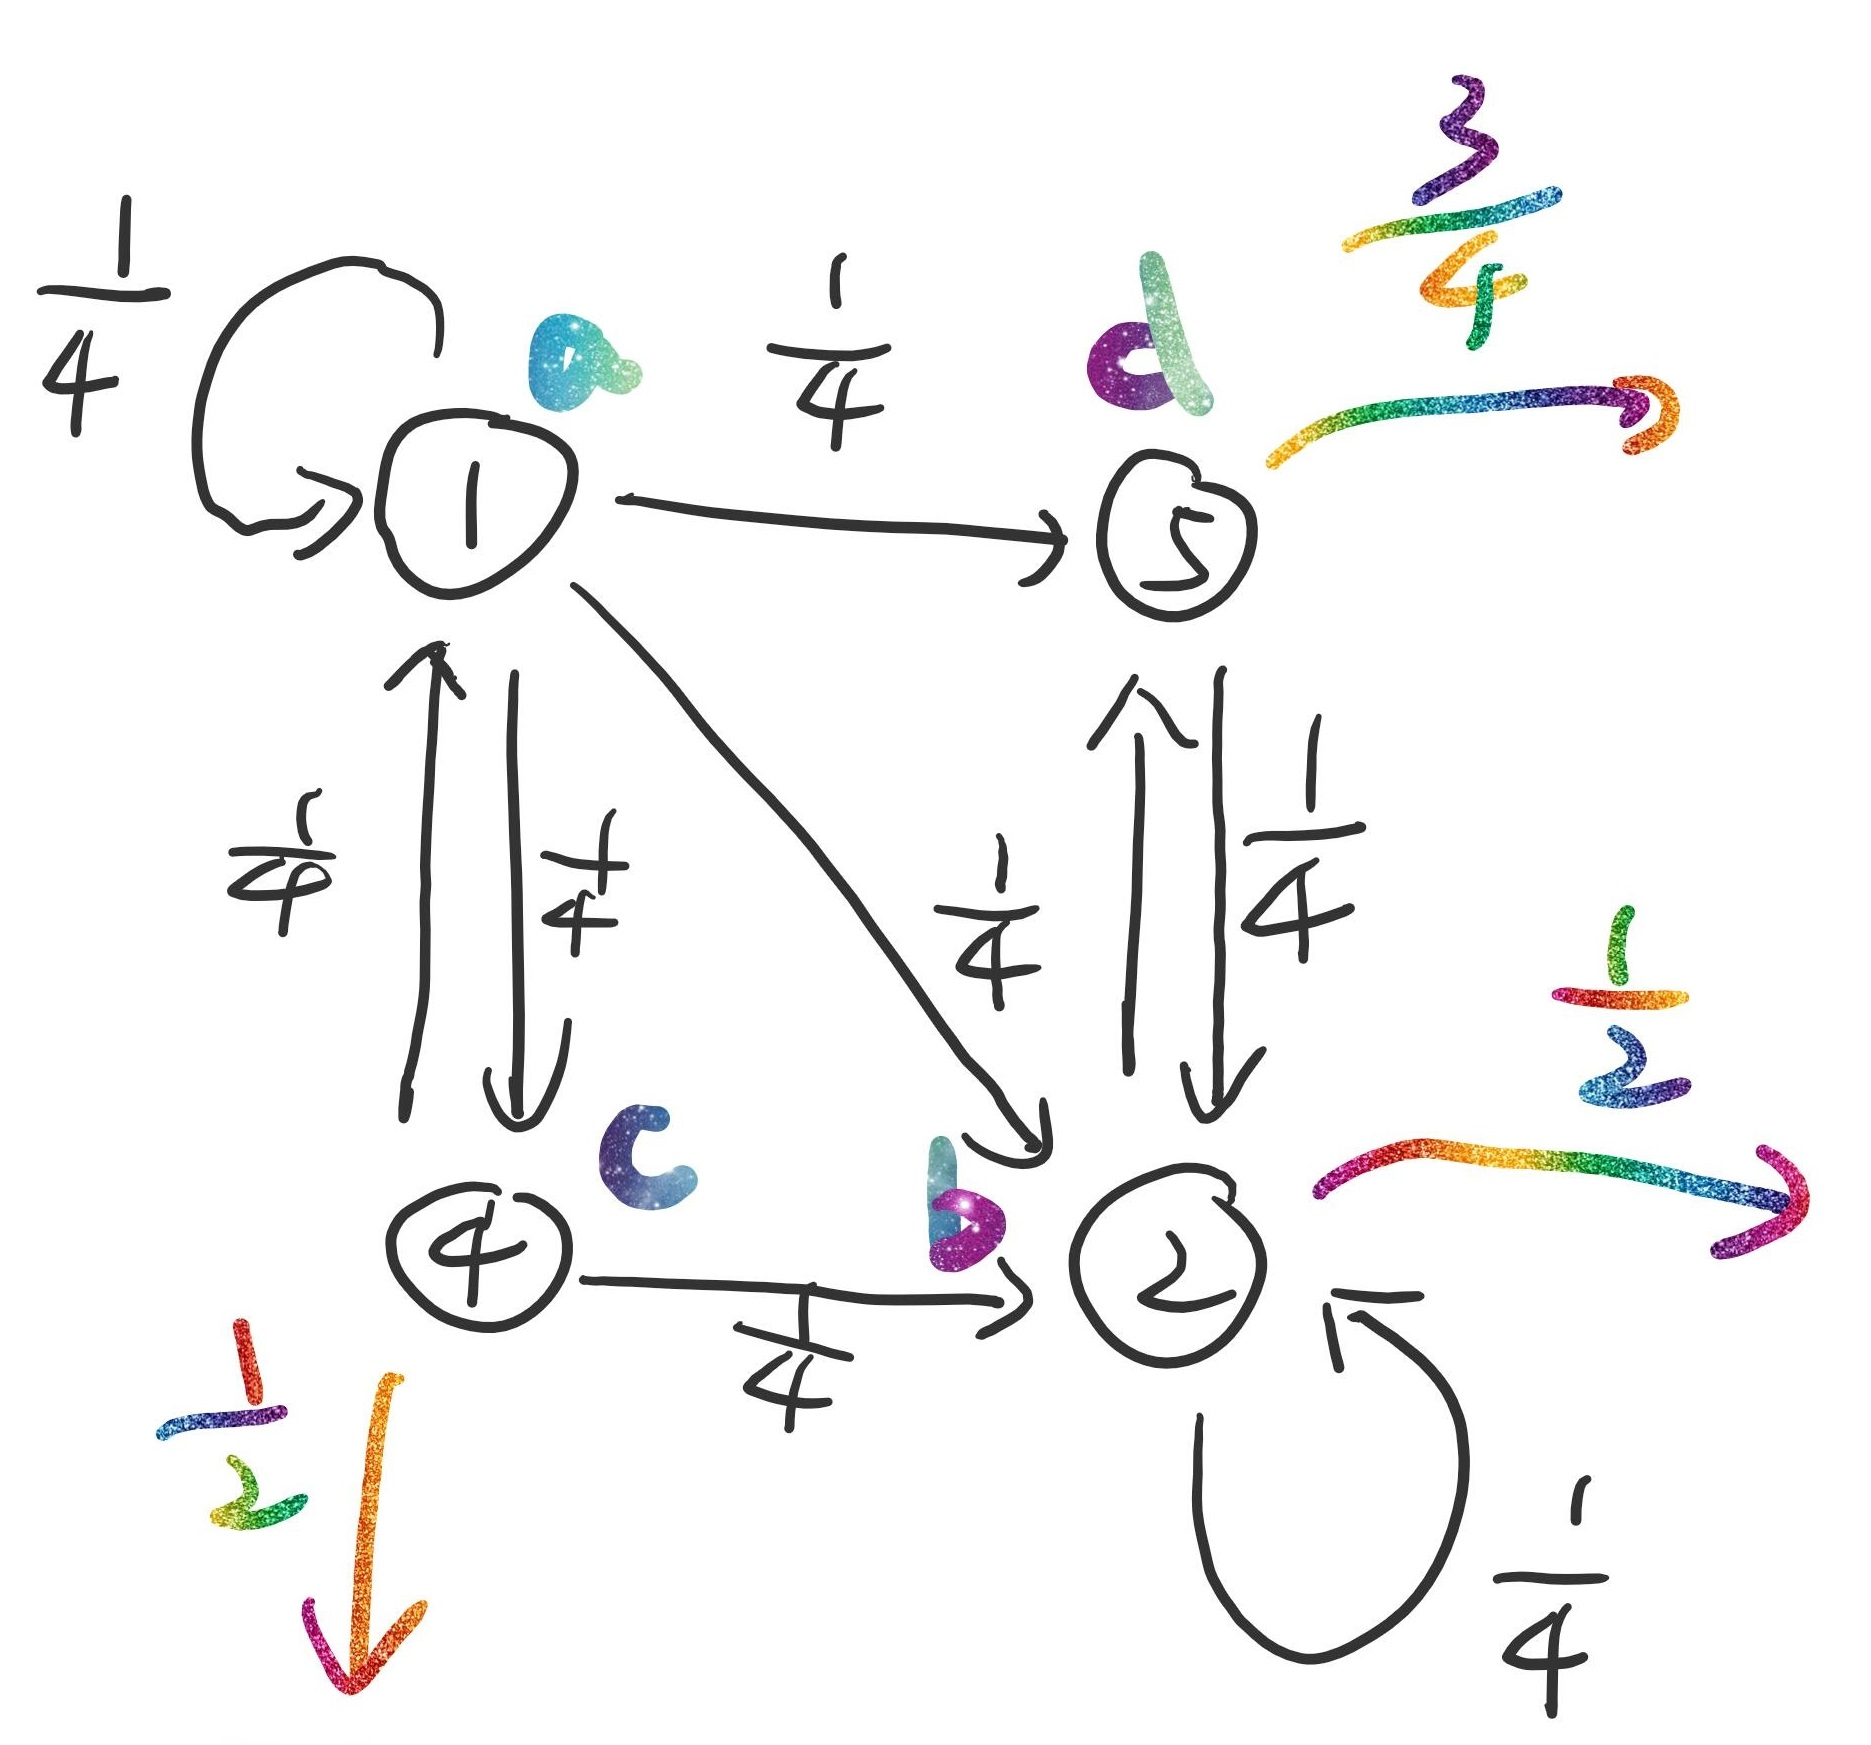
\includegraphics[width=0.4\textwidth]{figures/e33_p2.jpg}
  \end{center}
  Let $e_i$ be $\mathbb{E}(s_i \rightarrow T)$, then we have the equation set:
  $$
  \begin{cases}
  e_1 &=  1 + \frac{1}{4}e_1 + \frac{1}{4}e_2 + \frac{1}{4}e_4 + \frac{1}{4}e_5 \\
  e_2 &=  1 + \frac{1}{4}e_2 + \frac{1}{4}e_5 \\
  e_4 &=  1 + \frac{1}{4}e_1 + \frac{1}{4}e_2 \\
  e_5 &=  1 + \frac{1}{4}e_2 \\
  \end{cases}$$
  which can be expressed in the form of matrix:
  \begin{equation*}
  \left(
  \begin{array}{c}
  e_1 \\ e_2 \\ e_4 \\ e_5
  \end{array}
  \right) = \left(
  \begin{array}{c}
  1 \\ 1 \\ 1 \\ 1
  \end{array}
  \right) + \frac{1}{4} \times 
  \begin{pmatrix}
               1 &1 &1 &1 \\
                 &1 &  &1 \\
               1 &1 &  &  \\
                 &1 &  &  \\
  \end{pmatrix} \cdot 
  \left(
  \begin{array}{c}
  e_1 \\ e_2 \\ e_4 \\ e_5
  \end{array}
  \right)
  \end{equation*}
  The solution:
  \begin{equation*}
  \left(
  \begin{array}{c}
  e_1 \\ e_2 \\ e_4 \\ e_5
  \end{array}
  \right) = \frac{1}{121} \times \left(
  \begin{array}{c}
  384 \\ 220 \\ 272 \\ 176
  \end{array}
  \right)
  \end{equation*}
  Finally, let us calculate $\mathbb{E}(T)$. Toss coin $x$ and coin $y$ for the first time, and you will get four situations: $(x_1 = 0, y_1 = 0), (0 ,1), (1, 0), (1, 1)$. These $4$ sitations are equivalent to $s_1, s_2, s_4, s_5$ because what really matters in one state is the very last bit. \par
  $$
   \E(T) = 1 + \frac{e_1 + e_2 + e_4 + e_5}{4} = \frac{384}{121}
  $$

  %----------------------------3.3.2----------------------------
  \item The automaton will finally end up in 7 states, which can be divided into three categories.
\begin{enumerate}
  \item First Termination States: $1011$, where $10$ appears in $x$ (a) at the same time as $11$ appears in $y$
  \item Second Termination States: $1000, 1001, 1010$, where $10$ appears in $x$ (a) before $11$ appears in $y$
  \item Third Termination States: $0011, 0111, 1111$, where $10$ appears in $x$ (a) later than $11$ appears in $y$
\end{enumerate}
We denote these seven termination states $\{1011,1000,1001,1010,0011,0111,1111\}$ as $\{T_1, T_2, \cdots, T_7\}$. Also, we denote nine intermediate states $\{0000,0100,1100,0001\\,0101,1101,0010,0110,1110\}$ as $\{M_1, M_2, \cdots, M_9\}$. Consider the following probabilities: 
\begin{itemize}
  \item The probability of: at $t^{th}$ step we are at intermediate state $M_i$, which we denote as ${PM}_i^t$
  \item The probability of: after $t$ steps or before the $t^{th}$ step we terminate at termination state $T_i$, which we denote as ${PT}_i^t$
\end{itemize}
Define a vector $y^t$ to represent the overall probability at $t^{th}$ step:
$$y^t = \begin{bmatrix}PT_1^t\\\cdots\\PT_7^t\\PM_1^t\\\cdots\\PM_9^t \end{bmatrix}$$
At $t^{th}$ step, the system can either be at a intermediate state, or terminates at or even before the $t^{th}$ step. Therefore, the sum of each element in $y^t$ is always $1$.\\
Define transfer matrix for $y^t$ as $T$:
$$y^{t+1}=T\cdot y^t$$
And we the structure of $T$ is:
$$T = \begin{bmatrix}I&L_1\\O&L_2\end{bmatrix}$$
$I$ is a $7\times 7$ identity matrix, $O$ is a $9\times 7$ null matrix.\\
If there is no termination and keep tossing coins permanently, we can form a vector $y'^t$. Each element in it means the probability of the corresponding state in $t^{th}$ step. We then create the $16\times 16$ transfer matrix $T'$ for $y'^t$:
$$y'^{t+1}=T'\cdot y'^t$$
The sum of each column in $T'$ is 1. Then we take the last nine columns of $T'$ to form $\begin{bmatrix}L_1\\L_2\end{bmatrix}$.\\
The following figure shows the structure of $T$:
    \begin{figure}[htbp]
        \centering
        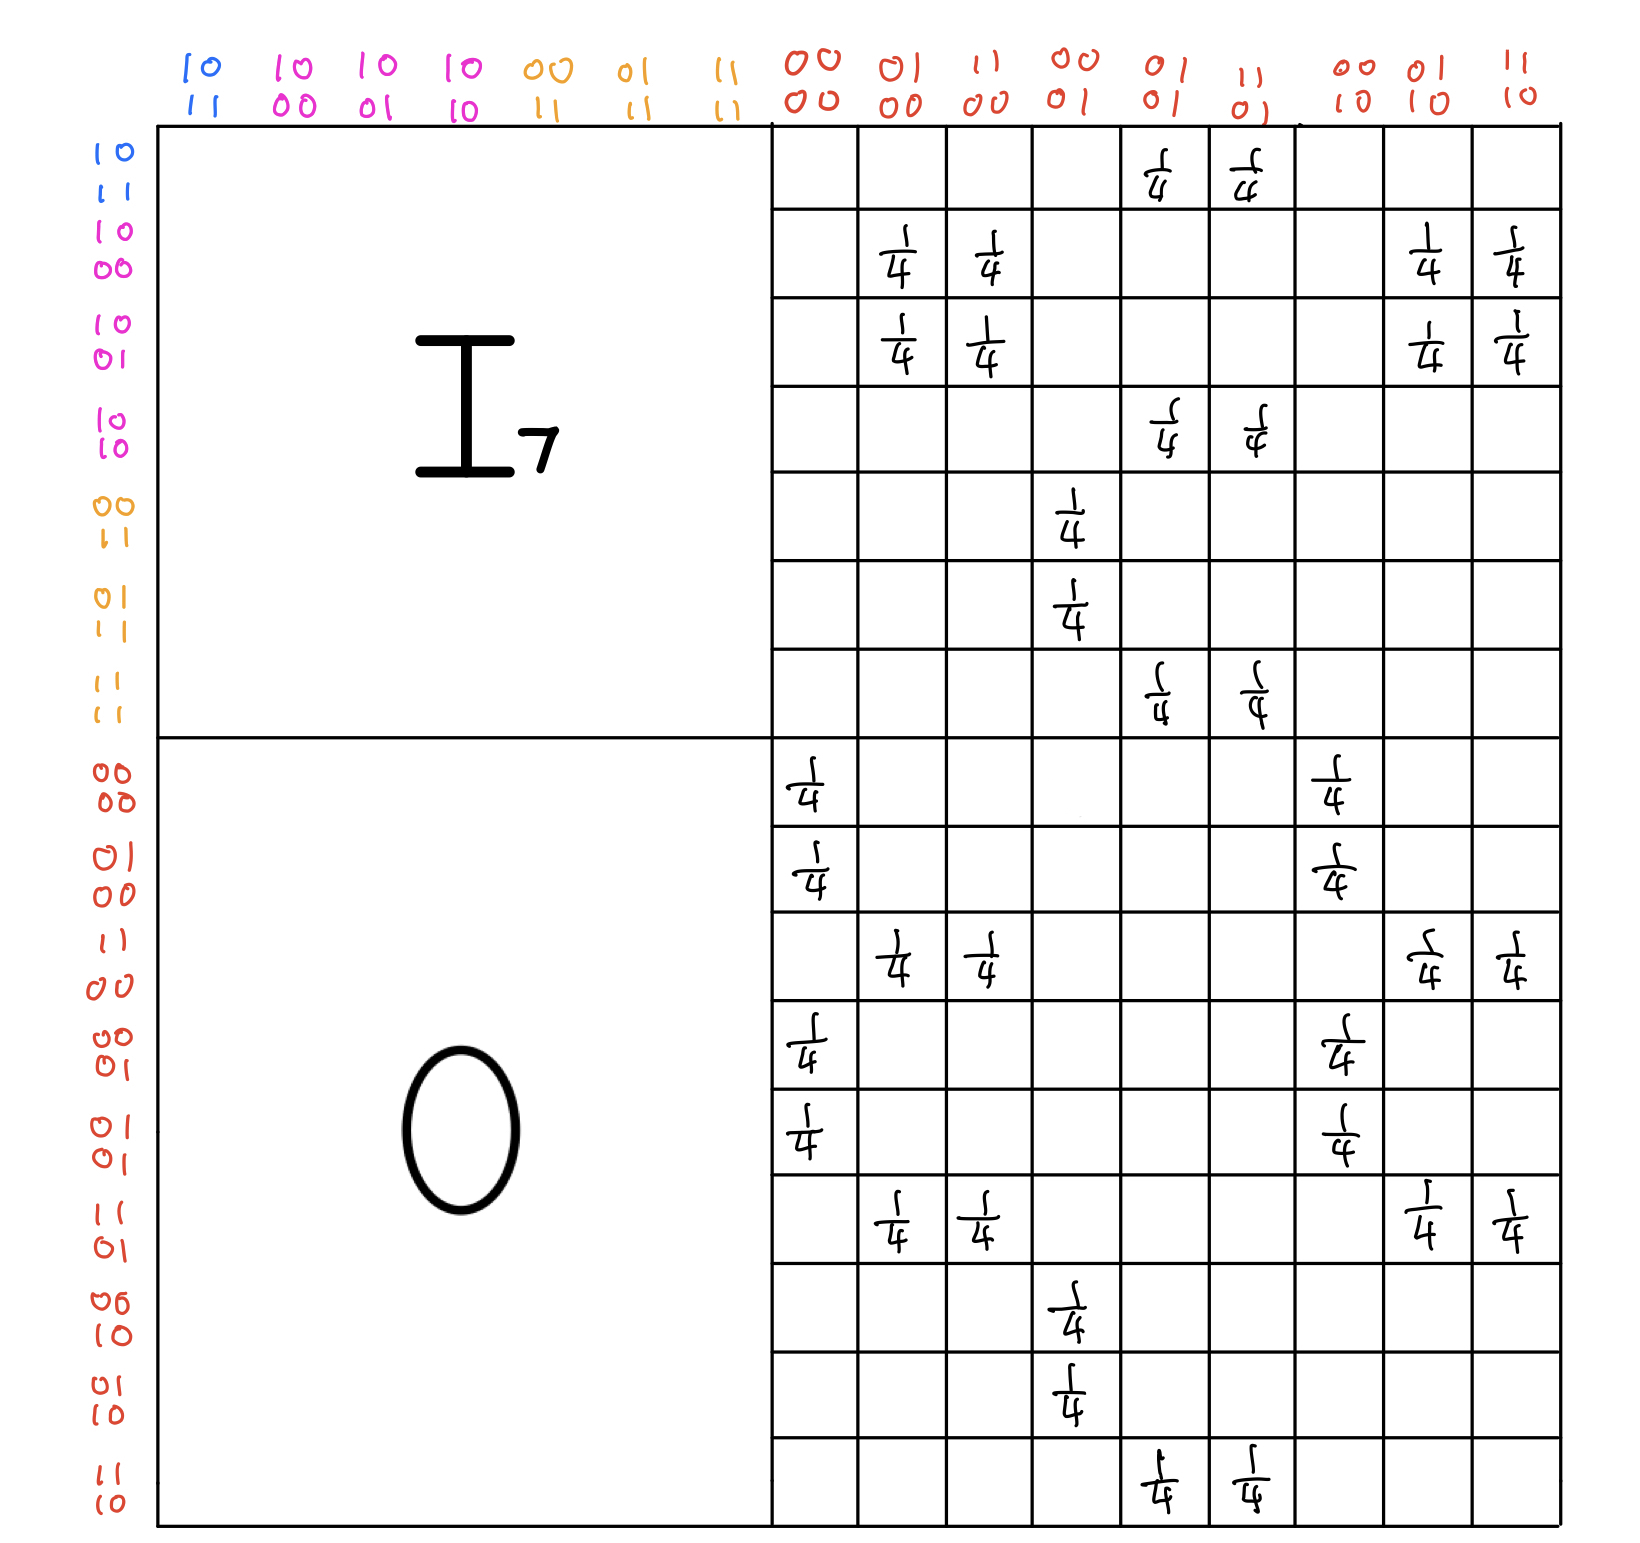
\includegraphics[width=0.9\textwidth]{figures/T-structure.jpeg}
        \caption{Structure of Matrix T}
    \end{figure}
Therefore, we get the the recurrence formula:
$$y^{n}=T^n\cdot y^0$$
$y^0$ is a one-hot vector, the $8^{th}$ element of which (corresponding to $0000$) is 1.
We use python to compute the result when n is approximate to infinity and we get:
$$\lim\limits_{n\to+\infty}y^n=\begin{bmatrix}17/121\\24/121\\24/121\\17/121\\11/121\\11/121\\17/121\\0\\\cdots\\0\end{bmatrix}$$
That is to say the system will finally terminate, the probability of end up in First Termination States is $17/121$, Second Termination States is $65/121$, Third  Termination States is $39/121$.
  \end{enumerate}
\end{solution}

\begin{exercise}
   Let us toss a biased coin, that is $1$ comes up with some probability $p \in [0,1]$. Let $T$ be the number
   of tosses until the first $1$ appears.
   \begin{enumerate}
        \item Give an explicit formula for $\E[T^2]$ in terms of $p$.
        \item Give an explicit formula for $\E\left[\frac{1}{T}\right]$ in terms of $p$.
   \end{enumerate}  
\end{exercise}

%----------------------------3.4.1----------------------------
\begin{solution}
Define $x=1-p$.
\begin{enumerate}
  \item
  \begin{equation}
    \begin{split}
      \E[T^2]&= \sum_{n=1}^\infty n^2(1-p)^{n-1}p\\
      &=p\sum_{n=1}^\infty n^2x^{n-1}\\
      &=p(\sum_{n=1}^\infty n(n-1)x^{n-1}+\sum_{n=1}^\infty nx^{n-1})\\
      &=px\sum_{n=1}^\infty (x^n)'')+p\sum_{n=1}^\infty (x^n)'\\
      &=px(\sum_{n=1}^\infty x^n)''+p(\sum_{n=1}^\infty (x^n))'\\
      &=px(\frac{2}{(1-x)^3})+p(\frac{1}{p^2})\\
      &=\frac{2-p}{p^2}
    \end{split}
  \end{equation}

%----------------------------3.4.2----------------------------
  \item

  \begin{equation}
    \begin{split}
      \E[\frac{1}{T}]&= \sum_{n=1}^\infty \frac{1}{n}(1-p)^{n-1}p\\
      &=p\sum_{n=1}^\infty \frac{x^{n-1}}{n}\\
      &=\frac{p}{1-p}(\sum_{n=1}^\infty \frac{x^n}{n})\\
      &=\frac{p}{1-p}(-ln(1-x))\\
      &=\frac{plnp}{p-1}
    \end{split}
  \end{equation}
\end{enumerate}
\end{solution}









\end{document}

